\documentclass[11pt]{report}

\usepackage{geometry}
\geometry{a4paper}
\usepackage{graphicx}
\graphicspath{ {./images/} }
\DeclareGraphicsExtensions{.png,.pdf,.jpg}

\title{Proyecto de Grado}
\author{Javier Ricardo Becerra Bedoya}

\begin{document}

\maketitle

\chapter{INTRODUCCIÓN}

Las enfermedades neurodegenerativas son un término general para una variedad de condiciones que afectan principalmente las neuronas del cerebro humano. Las neuronas son los componentes básicos del sistema nervioso central que incluye el cerebro y la medula espinal \cite{Neuro}. Las principales enfermedades neurodegenerativas son: Enfermedad de Alzheimer, Esclerosis lateral amiotrófica, Ataxia de Friedreich, Enfermedad de Huntington, Demencia con cuerpos de Lewy, Atrofia muscular espinal, Enfermedad de Parkinson, entre otras. En particular, la enfermedad de Parkinson es un trastorno neurodegenerativo que afecta predominantemente las neuronas productoras de dopamina en un área específica del cerebro llamada sustancia negra \cite{ParkFound}. Las personas que padecen esta enfermedad presentan los siguientes síntomas: temblor principalmente en reposo, lentitud de movimientos, rigidez en las extremidades, problemas en el equilibro y en la marcha \cite{ParkFound}.
\par
\medskip
\noindent
 Más de 10 millones de personas en el mundo viven con la enfermedad de Parkinson \cite{Estadistica}, alrededor de un millón en Estados Unidos \cite{Estadistica}. En Colombia, en ciudades como Bucaramanga, Medellín y Manizales, la prevalencia de la enfermedad de Parkinson es de 0.12\% al 0.47\% y proyectando estos datos a la población actual del país, se estima que podrían ser más de 22.000 casos \cite{colprensa}. La incidencia de la enfermedad de Parkinson aumenta con la edad, pero se estima que sólo el 4\% de los pacientes se diagnostican antes de los 50 años \cite{Estadistica}. Adicionalmente, alrededor de 60.000 estadounidenses son diagnosticados con Parkinson cada año \cite{Estadistica}. A partir de estos datos, se podría concluir que es importante desarrollar herramientas tecnológicas para la detección temprana de Parkinson, ya que esto podría mejorar la eficiencia de los tratamientos, así como la calidad de vida de los pacientes.
\par
\medskip
\noindent
El objetivo del reconocimiento de actividad es reconocer actividades humanas comunes en entornos de la vida real \cite{kim2010human}. El reconocimiento preciso de actividades es un desafío porque la actividad humana es compleja y altamanete diversa \cite{kim2010human}. La investigación en esta área emplea diferentes algoritmos de aprendizaje automático para reconocer actividades simples y complejas como caminar, correr, cocinar, etc \cite{cao2018gchar}. Particularmente, el reconocimiento de las actividades diarias es esencial para mantener un estilo de vida saludable, rehabilitación de pacientes y cambios de actividad entre los adultos mayores que pueden ayudar para detectar y diagnosticar enfermedades graves \cite{cao2018gchar}.
\par
\medskip
\noindent
Adicionalmente, los síntomas del Parkinson son poco entendidos. A los pacientes los afectan diversos factores de su vida diaria, como la calidad del sueño y la dieta. Para entender las diferencias, es necesario un monitoreo regular y constante por un tiempo prolongado. Lo que ocurre normalmente es que la gente asiste de una a dos veces a un especialista anualmente, lo que hace imposible un seguimiento continuo de la enfermedad \cite{elcomercio}. Debido a la baja frecuencia de monitoreo de la enfermedad en la actualidad, es importante el uso de herramientas tecnológicas que permitan hacer el monitoreo de la enfermedad de una manera continua, para extraer mayor información.
\par
\medskip
\noindent
Por lo tanto, el objetivo de este trabajo de investigación es Implementar un sistema de clasificación de actividad humana a partir de señales de acelerómetros para posteriores estudios en pacientes con Parkinson.
\par
\medskip
\noindent
El diagrama de bloques que representa el desarrollo del proyecto es el siguiente:
\begin{figure}[h]
  \centering
    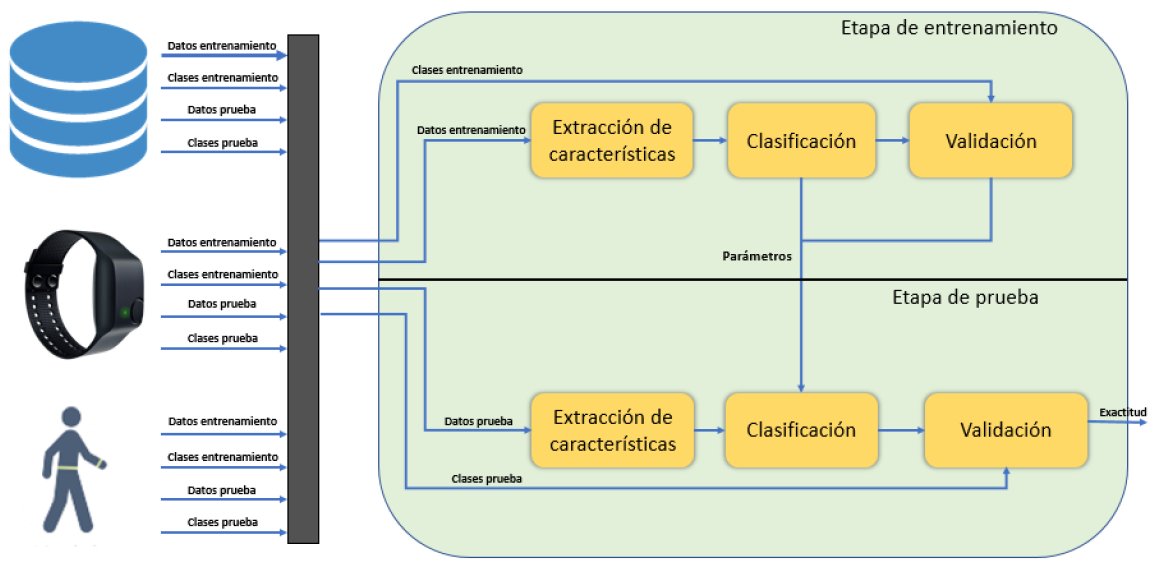
\includegraphics[width=1\textwidth]{diagrama}
   \caption{Diagrama de Bloques del Sistema}
\end{figure}

\chapter{MARCO TEÓRICO}
A lo largo de este capítulo se pretende mostrar los conceptos básicos del análisis de clasificación de actividad humana,
así como las técnicas y tecnologías que han permitido su desarrollo y aplicación durante los últimos años.
\par
\medskip
\noindent
Primero, se dará una introducción al concepto de clasificación de actividad humana y del porqué se ha convertido en una herramienta
de importancia en el análisis médico y de ingeniería en la actualidad. Posteriormente, se explicará detalladamente los métodos usados para el reconocimiento de actividad humana y cuáles son los últimos avances en el tema. Se repasarán aplicaciones útiles ya trabajadas en anteriores trabajos en el campo de acción de la ingeniería.
\section{Antecedentes}
En noviembre 07 del 2012 el departamento de medicina física y de rehabilitación, de la Universidad Northwestern
en Chicago publicó un artículo llamado “Using mobile phones for activity recognition in Parkinson’s patients” en
el cual expone el trabajo realizado que consistió en identificar 5 actividades (caminando, reposo, sentado, de pie,
o no utilizando el celular) de 18 sujetos sanos y 8 pacientes con enfermedad de Parkinson. Además, se mostraban
las diferencias que hay entre los algoritmos de reconocimiento de actividad corporal entre personas sanas y
pacientes. Los resultados del proyecto arrojaron una exactitud del 96,1 \% de clasificación de actividades en las
personas sanas y un 92,2 \% en los pacientes. 
\par
\medskip
\noindent
En cuanto a los mecanismos de monitoreo de pacientes con Parkinson, se encuentra una aplicación móvil llamada
CloudUPDRS, es un sistema de análisis de datos que pueden usar los pacientes y sus cuidadores para evaluar con
precisión los síntomas motores de Parkinson. Se puede analizar movimientos como temblor, marcha y la capacidad
con la que interactúan con el Smartphone, para evaluar con precisión los síntomas de la enfermedad usando el
método UPDRS (Unified Parkinson’s Disease Rating Scale). Tiene la capacidad de descartar información falsa al
92,5\% \cite{PacientesParkinson}.
\par
\medskip
\noindent
Existe un sistema llamado Mobility Lab de APDM el cual pretende medir la progresión longitudinal de la
enfermedad de Parkinson. Analizan el equilibrio y la marcha de los pacientes ya que son los dos impedimentos
motores que más afectan la calidad de vida de los enfermos con Parkinson. Utilizan unos sensores llamados Opal,
que se localizan en las piernas, el tronco y los brazos, durante las dos actividades prescritas. Este sistema es una
aplicación futura debido a las medidas fiables que se pueden realizar con estos sensores \cite{MobilityLab}.
\par
\medskip
\noindent
Adicionalmente, en un proyecto realizado por un grupo de universidades latinoamericanas y liderado por Mónica
Huerta, con el título “Monitoreo remoto de pacientes con la enfermedad de Parkinson”, se pretendía mejorar el
diagnóstico y monitoreo de la enfermedad \cite{MonitoreoRemoto}. Usaron en la investigación un sensor de Kinect, smartphones,
hardware libre y smartwatch. Para cada dispositivo diseñaron una solución de monitoreo de la enfermedad. Es un
avance para proyectos futuros aplicados a la biomedicina, especialmente en enfermedades motoras.
\par
\medskip
\noindent
Finalmente, motivados por la necesidad de detectar automáticamente las diferentes actividades humanas, la
plataforma Kaggle lanzó en el 2016 un concurso abierto \cite{Kaggle}. Para esto, pusieron a disposición una base de datos
de señales de acelerómetros, correspondientes a 6 actividades de 30 personas. Grupos de diferentes partes del
mundo, desarrollaron métodos de clasificación de actividad humana, obteniendo 98\% de exactitud entre los
resultados más destacados.
\section{Algoritmos de Inteligencia artificial en HAR}
En las últimas décadas, un cambio drástico cambió la manera en la que almacenamos, percibimos y procesamos los datos. Una cantidad gigante de datos es generada cada segundo y si se analiza eficientemente estos datos pueden revelar importante información. Una parte importante en la predicción es seleccionar modelos adecuados \cite{ApplicationHAR}. Uno de los objetivos del proyecto es implementar los siguientes algoritmos en Matlab y analizar cuál es el más eficiente a la hora de clasificar actividad humana.
\begin{figure}[h]
  \centering
    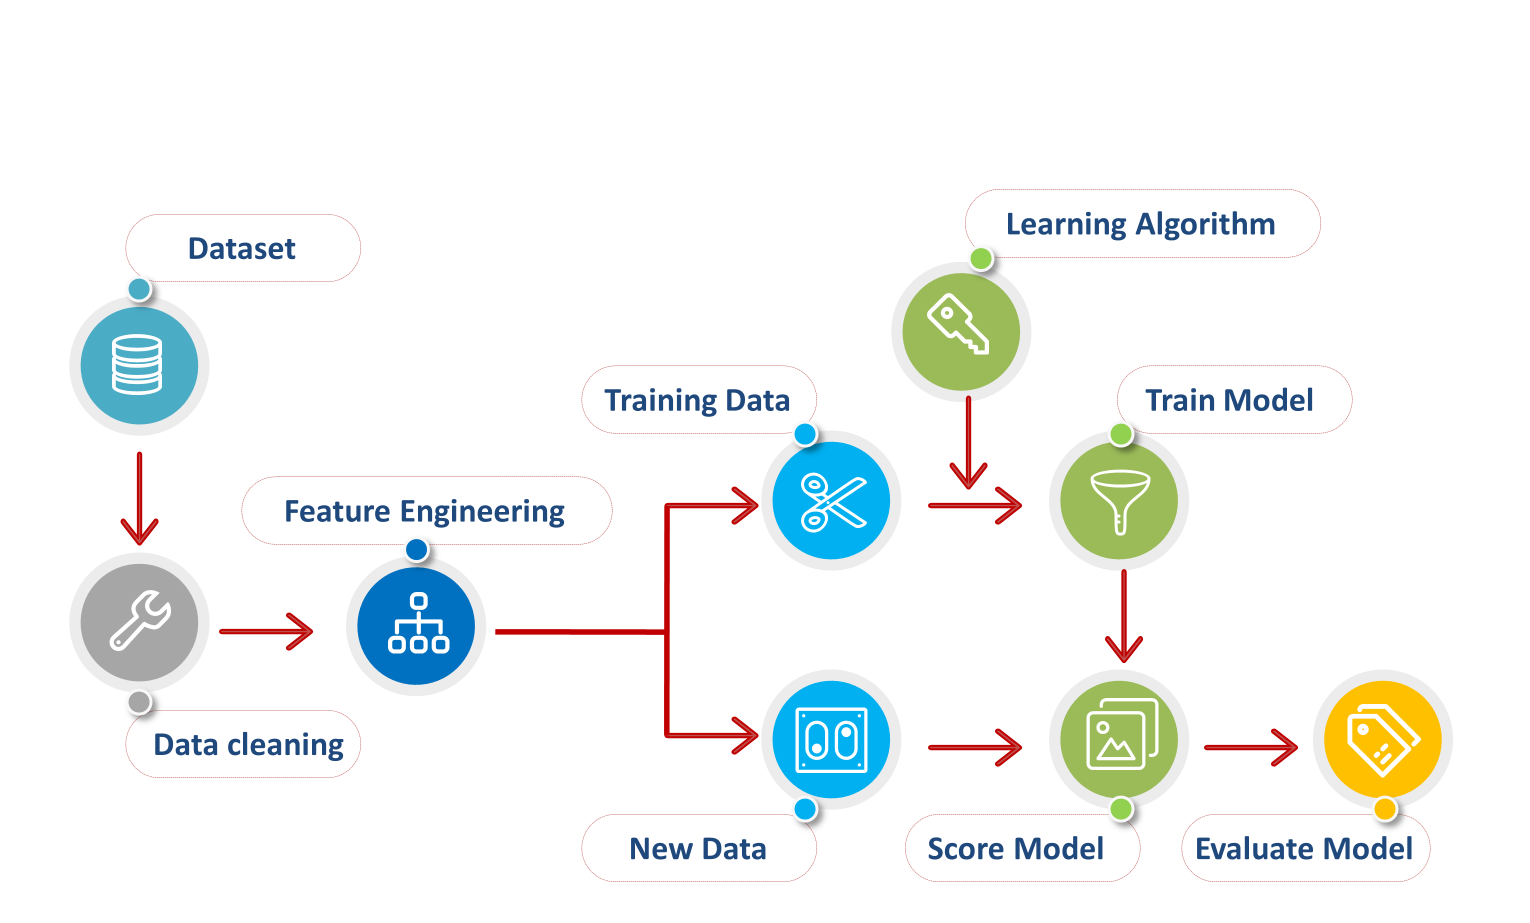
\includegraphics[width=0.5\textwidth]{machinelearning}
   \caption{Diagrama de Bloques de un sistema de Machine Learning \cite{huang}}
\end{figure}
\subsection {Árbol de decisiones}
\begin{figure}[h]
  \centering
    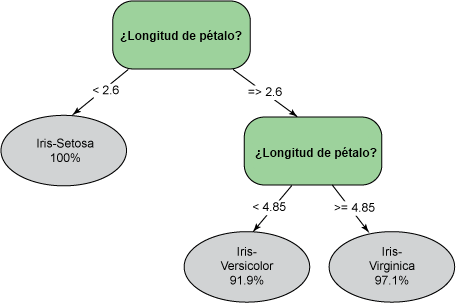
\includegraphics[width=0.5\textwidth]{decision}
   \caption{Ejemplo Árbol de Decisiones \cite{decisiont}}
\end{figure}
 Un árbol de decisión es un modelo de predicción. Dado un conjunto de datos se fabrican diagramas de construcciones lógicas, que sirven para representar y categorizar una serie de condiciones que ocurren de forma sucesiva, para la resolución de un problema. Los árboles de decisión están formados por nodos, vectores de números, flechas y etiquetas. Cada nodo se puede definir como el momento en el que se ha de tomar una decisión de entre varias posibles, lo que va haciendo que a medida que aumenta el número de nodos aumente el número de posibles finales a los que puede llegar el individuo. Los vectores de números serían la solución final a la que se llega en función de las diversas posibilidades que se tienen, dan las utilidades en esa solución. Las flechas son las uniones entre un nodo y otro y representan cada acción distinta. Las etiquetas se encuentran en cada nodo y cada flecha y dan nombre a cada acción \cite{ApplicationHAR}.
\subsection {Random Forests}
Es un clasificador que consiste en una colección independiente, idénticamente distribuida y al azar de clasificadores organizados en árboles, en donde cada árbol aporta un único voto a la clase más popular de X. Básicamente, para los agrupamientos Random Forests selecciona al azar un subconjunto de los atributos para luego volver a seleccionar el mejor corte entre estos. Posteriormente el proceso se repite en cada uno de los árboles (muchos árboles crecen de la misma manera) para así construir un bosque. Finalmente todos los árboles son usados en el resultado final a partir del promedio de los resultados de cada uno de los árboles \cite{ApplicationHAR}.
\begin{figure}[h]
  \centering
    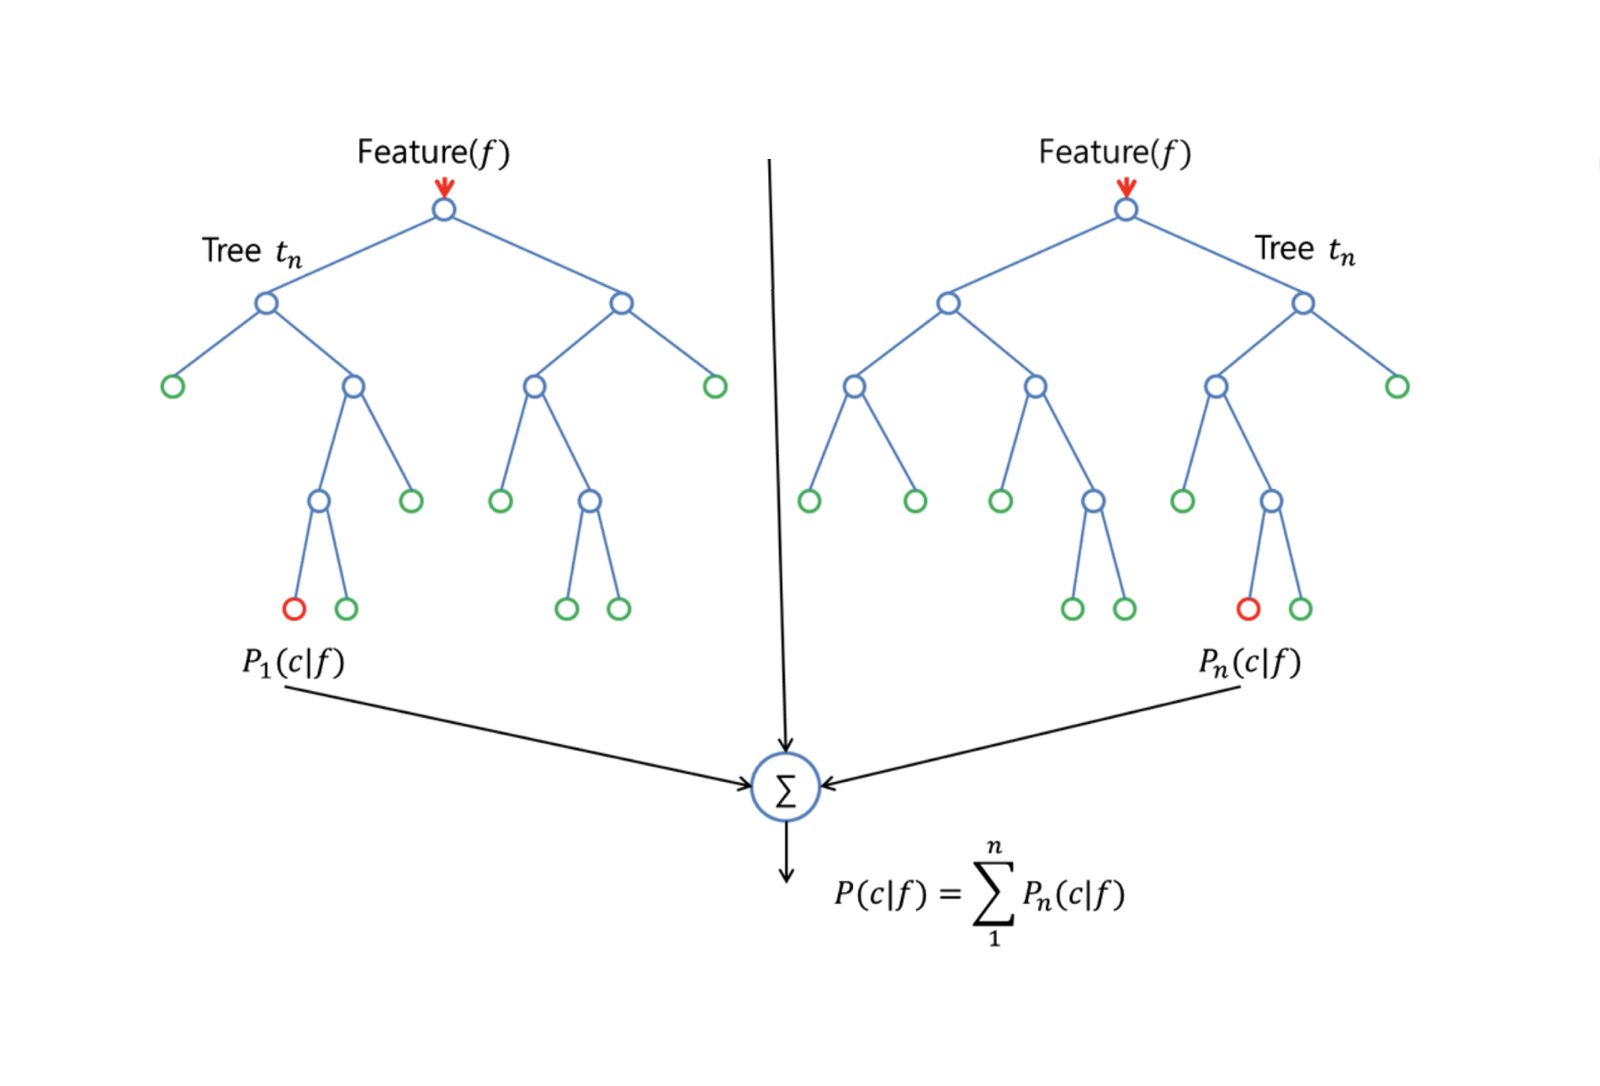
\includegraphics[width=0.5\textwidth]{random}
   \caption{Ejemplo Random Forest \cite{randomf}}
\end{figure}  
\subsection {Support Vector Machine}
\begin{figure}[h]
  \centering
    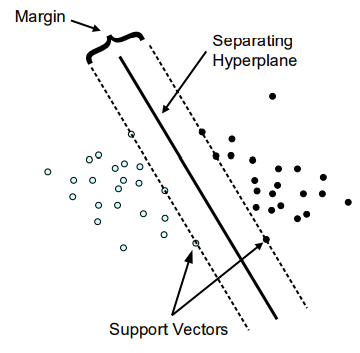
\includegraphics[width=0.5\textwidth]{support}
   \caption{Ejemplo Random Forest \cite{supportv}}
\end{figure}
Son un conjunto de algoritmos de aprendizaje supervisado. Estos métodos están propiamente relacionados con problemas de clasificación y regresión. Dado un conjunto de ejemplos de entrenamiento (de muestras) podemos etiquetar las clases y entrenar una SVM es un modelo que representa a los puntos de muestra en el espacio, separando las clases a 2 espacios lo más amplios posibles mediante un hiperplano de separación definido como el vector entre los 2 puntos, de las 2 clases, más cercanos al que se llama vector sporte. Cuando las nuevas muestras se ponen en correspondencia con dicho modelo, en función de los espacios a los que pertenezcan, pueden ser clasificadas a una o la otra clase \cite{ApplicationHAR}.
\bibliography{biblio} 
\bibliographystyle{ieeetr}

\end{document}